\documentclass{article}
\usepackage{amsmath,mathtools}
\usepackage{amssymb}
\usepackage{xargs}
\usepackage[dvipsnames]{xcolor}
\usepackage[margin=1.2in]{geometry}
\usepackage{graphicx}
\usepackage{enumitem}
\usepackage{pgfplots, pgfplotstable}
\usetikzlibrary{arrows.meta,bending,datavisualization.formats.functions,decorations.markings,decorations.pathmorphing}
\usepgfplotslibrary{fillbetween}
\usetikzlibrary{patterns}
\usepackage{tikz}
\usepackage[skins,theorems]{tcolorbox}
\tcbset{highlight math style={enhanced,
  colframe=blue,colback=white,arc=0pt,boxrule=1pt}}

\tikzset{% inspired by https://tex.stackexchange.com/a/316050/121799
  arc arrow/.style args={to pos #1 with length #2 and options #3}{
  decoration={
      markings,
       mark=at position 0 with {\pgfextra{%
       \pgfmathsetmacro{\tmpArrowTime}{#2/(\pgfdecoratedpathlength)}
       \xdef\tmpArrowTime{\tmpArrowTime}}},
      mark=at position {#1-\tmpArrowTime} with {\coordinate(@1);},
      mark=at position {#1-2*\tmpArrowTime/3} with {\coordinate(@2);},
      mark=at position {#1-\tmpArrowTime/3} with {\coordinate(@3);},
      mark=at position {#1} with {\coordinate(@4);
      \draw[-{Stealth[length=#2,bend,#3]}]       
      (@1) .. controls (@2) and (@3) .. (@4);},
      },
   postaction=decorate,
   }
}

\newenvironment{sysmatrix}[1]
 {\left[\begin{array}{@{}#1@{}}}
 {\end{array}\right]}
\newcommand{\ro}[1]{%
  \xrightarrow{\mathmakebox[\rowidth]{#1}}%
}
\newlength{\rowidth}% row operation width
\AtBeginDocument{\setlength{\rowidth}{3em}}

\begin{document}

\title{Differential Equations HW \#4}
\author{Ozaner Hansha}
\date{November 12, 2019}
\maketitle

\newcommandx{\der}[2][1=y, 2=t]{\frac{d#1}{d#2}}
\newcommand*\eval[3]{\left[#1\right]_{#2}^{#3}}
\renewcommand{\vec}[1]{\mathbf{#1}}
\newcommand*\tr[1]{\text{tr}\left(#1\right)}

\section*{Problem 1}
\noindent\textbf{Problem:} Let $\vec y_1(t)$ and $\vec y_2(t)$ be solutions to the following system:

\begin{equation*}
  \der[\vec y]=\underbrace{\begin{bmatrix}
    a&b\\c&d
  \end{bmatrix}}_{\vec A}\vec y
\end{equation*}

And let $D(t)=\det[\vec y_1(t)\quad\vec y_1(t)]$

\begin{enumerate}[label=\textbf{\alph*})]
  \item Show that $D(t)$ satisfies $\der[D]=\tr{\vec A} D$.
  \item Show that if $\vec y_1(0)$ and $\vec y_2(0)$ are linearly independent, then $\vec y_1(t)$ and $\vec y_2(t)$ are linearly independent for all $t$.
\end{enumerate}
\bigskip

\noindent\textbf{Solution:} \textbf{a)} First notice the following:
\begin{align*}
  \vec y_1'&=A\vec y_1\\
  \begin{bmatrix}
    y_{11}'\\y_{21}'
  \end{bmatrix}&=\begin{bmatrix}
    ay_{11}+by_{21}\\cy_{11}+dy_{21}
  \end{bmatrix}\tag{Eq. 1}\\
  \vec y_2'&=A\vec y_2\\
  \begin{bmatrix}
    y_{12}'\\y_{22}'
  \end{bmatrix}&=\begin{bmatrix}
    ay_{12}+by_{22}\\cy_{12}+dy_{22}
  \end{bmatrix}\tag{Eq. 2}
\end{align*}

Now consider $D(t)$:
\begin{align*}
  D(t)&=\det[\vec y_1(t)\quad\vec y_1(t)]\\
  &=\begin{vmatrix}
    y_{11}&y_{12}\\y_{21}&y_{22}
  \end{vmatrix}=y_{11}y_{22}-y_{12}y_{21}
\end{align*}

We can now see that $D$ does indeed satisfy the given ODE:
\begin{align*}
  \der[D]&=y_{11}'y_{22}+y_{11}y_{22}'-y_{12}'y_{21}-y_{12}y_{21}'\tag{product rule}\\
  &=y_{22}(ay_{11}+by_{21})+y_{11}(cy_{12}+dy_{22})-y_{21}(ay_{12}+by_{22})-y_{12}(cy_{11}+dy_{21})\tag{Eq. 1 \& 2}\\
  &=(ay_{11}y_{22}-ay_{12}y_{21})+(by_{21}y_{22}-by_{22}y_{21})+(cy_{12}y_{11}-cy_{11}y_{12})+(dy_{22}y_{11}-dy_{21}y_{12})\\
  &=a\underbrace{\begin{vmatrix}y_{11}&y_{12}\\y_{21}&y_{22}\end{vmatrix}}_{=D}+b\underbrace{\begin{vmatrix}y_{21}&y_{22}\\y_{21}&y_{22}\end{vmatrix}}_{=0}+c\underbrace{\begin{vmatrix}y_{12}&y_{11}\\y_{12}&y_{11}\end{vmatrix}}_{=0}+d\underbrace{\begin{vmatrix}y_{11}&y_{12}\\y_{21}&y_{22}\end{vmatrix}}_{=D}\\
  &=(a+d)D=\tr{\vec A}D
\end{align*}

% And so $D(t)$ is indeed a solution to the ODE.
% \bigskip

\textbf{b)} Note that our two functions $\vec y_1(t)$ and $\vec y_2(t)$ are linearly dependent if and only if:
\begin{equation*}
  (\exists k_1,k_2)(\forall t)\,\,\,\,\,k_1\vec y_1(t)=k_2\vec y_2(t)\tag{*}
\end{equation*}

However if $\vec y_1(0)$ and $\vec y_2(0)$ are not linearly dependent, i.e. linearly \textit{in}dependent, then the following is the case:
\begin{equation*}
  (\nexists k_1,k_2)\,\,\,\,\,k_1\vec y_1(0)=k_2\vec y_2(0)
\end{equation*}

And so statement (*) does not hold and thus, $\vec y_1(t)$ and $\vec y_2(t)$ are not linearly dependent. In other words, they are linearly \textit{in}dependent.

\section*{Problem 2}
\noindent\textbf{Problem:} Solve the following IVP:

\begin{equation*}
  \der[\vec y]=\underbrace{\begin{bmatrix}
    -2&-2\\-2&1
  \end{bmatrix}}_{\vec A}\vec y,\quad \vec y(0)=\begin{bmatrix}
    1\\2
  \end{bmatrix}
\end{equation*}

\noindent\textbf{Solution:} To find a spanning set of solutions, we first find the eigenvalues of $\vec A$:
\begin{align*}
  0&=\det(\vec A-\lambda \vec I)\\
  &=\begin{vmatrix} -2-\lambda & -2 \\ -2 & 1-\lambda \end{vmatrix}\\
  &=(1-\lambda)(-2-\lambda)-4\\
  &=\lambda^2+\lambda-6\\
  &=(\lambda+3)(\lambda-2)\\
  &\longrightarrow \begin{cases}
    \lambda_1=2\\
    \lambda_2=-3
  \end{cases}
\end{align*}

Now we must find an eigenvector, $\vec v_1$ and $\vec v_2$ respectively, corresponding to each eigenvalue. To do this, we find the eigenspaces corresponding to each eigenvalue, starting with $\lambda_1$:
\begin{align*}
  E_1(\vec A)&=\text{Null}(\vec A-\lambda_1\vec I)\\
&=\text{Null}\begin{bmatrix} -4 & -2 \\ -2 & -1 \end{bmatrix}\\
&=\text{Null}\begin{bmatrix} 2 & 1 \\ 0 & 0 \end{bmatrix}\tag{ref}\\
&=\text{Span}\left\{\begin{bmatrix} 1\\-2\end{bmatrix}\right\}\tag{$x_2=-2x_1$}\\
&\stackrel{\text{let}}{\longrightarrow} \vec v_1=\begin{bmatrix} 1\\-2\end{bmatrix}
\end{align*}

Now we do the same for $\lambda_2$:
\begin{align*}
  E_2(\vec A)&=\text{Null}(\vec A-\lambda_2\vec I)\\
&=\text{Null}\begin{bmatrix} 1 & -2 \\ -2 & 4 \end{bmatrix}\\
&=\text{Null}\begin{bmatrix} 1 & -2 \\ 0 & 0 \end{bmatrix}\tag{ref}\\
&=\text{Span}\left\{\begin{bmatrix} 2\\1\end{bmatrix}\right\}\tag{$x_1=2x_2$}\\
&\stackrel{\text{let}}{\longrightarrow} \vec v_2=\begin{bmatrix} 2\\1\end{bmatrix}
\end{align*}

And so we have, for our desired solution $\vec y(t)$, the following:
\begin{align*}
  \vec y(t)&=k_1e^{\lambda_1t}\vec v_1+k_2e^{\lambda_2t}\vec v_2\tag{distinct roots}\\
  \vec y(0)&=k_1e^0\vec v_1+k_2e^0\vec v_2\tag{let $t=0$}\\
  \begin{bmatrix}
    1\\2
  \end{bmatrix}&=k_1\begin{bmatrix} 1\\-2\end{bmatrix}+k_2\begin{bmatrix} 2\\1\end{bmatrix}
\end{align*}

We can represent this system as the following augmented matrix:
\begin{align*}
  \begin{sysmatrix}{rr|r}
      1 & 2 & 1 \\
      -2 & 1 & 2 \\
  \end{sysmatrix}&\ro{r_2+2r_1}
  \begin{sysmatrix}{rr|r}
      1 & 2 & 1 \\
      0 & 5 & 4 \\
  \end{sysmatrix}\\
  &\ro{(1/5)r_2}
  \begin{sysmatrix}{rr|r}
      1 & 2 & 1 \\
      0 & 1 & 4/5 \\
  \end{sysmatrix}\\
  &\ro{r_1-2r_2}
  \begin{sysmatrix}{rr|r}
      1 & 0 & -3/5 \\
      0 & 1 & 4/5 \\
  \end{sysmatrix}
\end{align*}

And so $k_1=\frac{-3}{5}$ and $k_2=\frac{4}{5}$ giving us our desired solution:
\begin{align*}
  \vec y(t)&=k_1e^{\lambda_1t}\vec v_1+k_2e^{\lambda_2t}\vec v_2\\
  &=\frac{-3}{5}e^{2t}\begin{bmatrix} 1\\-2\end{bmatrix}+\frac{4}{5}e^{-3t}\begin{bmatrix} 2\\1\end{bmatrix}\\
  &=\tcbhighmath[boxrule=0.4pt,colframe=blue,colback=blue!10!white]{\frac{1}{5}\begin{bmatrix}
    -3e^{2t}+8e^{-3t}\\
    6e^{2t}+4e^{-3t}
  \end{bmatrix}}
\end{align*}

\section*{Problem 3}
\noindent\textbf{Problem:} Find the general solution to the following system:

\begin{equation*}
  \der[\vec y]=\underbrace{\begin{bmatrix}
    -3&-5\\3&1
  \end{bmatrix}}_{\vec A}\vec y
\end{equation*}

\noindent\textbf{Solution:} To find a spanning set of solutions, we first find the eigenvalues of $\vec A$:
\begin{align*}
  0&=\det(\vec A-\lambda \vec I)\\
  &=\begin{vmatrix} -3-\lambda & -5 \\ 3 & 1-\lambda \end{vmatrix}\\
  &=(1-\lambda)(-3-\lambda)+15\\
  &=\lambda^2+2\lambda+12\\
  &\longrightarrow \lambda=\frac{-2\pm\sqrt{4-48}}{2}\tag{quadratic formula}\\
  &\longrightarrow \begin{cases}
    \lambda_1=-1+i\sqrt{11}\\
    \lambda_2=-1-i\sqrt{11}
  \end{cases}
\end{align*}

Now we must find an eigenvector $\vec v$ that corresponds to one of the eigenvalues. To do this, we find the eigenspace corresponding to, say, $\lambda_2$:
\begin{align*}
  E_2(\vec A)&=\text{Null}(\vec A-\lambda_2\vec I)\\
&=\text{Null}\begin{bmatrix} -2+i\sqrt{11} & -5 \\ 3 & 2+i\sqrt{11} \end{bmatrix}
\end{align*}

This is equivalent to the solution set of the following system of equations:
\begin{equation*}
  \begin{cases}
    (-2+i\sqrt{11})v_1=5v_2\\
    3v_1=(-2-i\sqrt{11})v_2
  \end{cases}
\end{equation*}

Via substitution we find:
\begin{align*}
  (-2-i\sqrt{11})v_2&=\frac{5\cdot3}{-2+i\sqrt{11}}\\
  v_2&=\frac{15}{(-2-i\sqrt{11})(-2+i\sqrt{11})}=1
\end{align*}

Plugging this into the second equation we find:
\begin{equation*}
  v_1=\frac{-1}{3}(2+i\sqrt{11})
\end{equation*}

And so our eigenspace is given by:
\begin{equation*}
  E_2(\vec A)=\text{Span}\left\{\begin{bmatrix}
    \frac{-1}{3}(2+i\sqrt{11})\\1
  \end{bmatrix}\right\}
\end{equation*}

And so, for ease of calculation, we'll let the following be our vector $\vec v$:
\begin{equation*}
  \vec v=\begin{bmatrix}
    2+i\sqrt{11}\\-3
  \end{bmatrix}
\end{equation*}

Now consider the following particular solution to the system:
\begin{align*}
  \vec y_p(t)&=e^{(-1-i\sqrt{11})t}\vec v\tag{straight line solution}\\
  &=e^{-t}e^{-it\sqrt{11}}\vec v\\
  &=e^{-t}(\cos -t\sqrt{11}+i\sin -t\sqrt{11})\vec v\tag{Euler's formula}\\
  &=e^{-t}\cos(t\sqrt{11})-e^{-t}i\sin(t\sqrt{11})\begin{bmatrix}
    2+i\sqrt{11}\\-3
  \end{bmatrix}\\
  &=\begin{bmatrix}
    2e^{-t}\cos(t\sqrt{11})-2ie^{-t}\sin(t\sqrt{11})+ie^{-t}\sqrt{11}\cos(t\sqrt{11})+e^{-t}\sqrt{11}\sin(t\sqrt{11})\\-3e^{-t}\cos(t\sqrt{11})+3e^{-1}i\sin(t\sqrt{11})
  \end{bmatrix}\\
  &=\underbrace{\begin{bmatrix}
    2e^{-t}\cos(t\sqrt{11})+e^{-t}\sqrt{11}\sin(t\sqrt{11})\\-3e^{-t}\cos(t\sqrt{11})
  \end{bmatrix}}_{\vec y_\mathcal R(t)}
  +i\underbrace{\begin{bmatrix}
    -2e^{-t}\sin(t\sqrt{11})+e^{-t}\sqrt{11}\cos(t\sqrt{11})\\3e^{-t}\sin(t\sqrt{11})
  \end{bmatrix}}_{\vec y_\mathcal I(t)}
\end{align*}

And so the general real solution to the system is given by:
\begin{align*}
  \vec y(t)&=k_1\vec y_\mathcal R(t)+k_2\vec y_\mathcal I(t)\\
  &=\tcbhighmath[boxrule=0.4pt,colframe=blue,colback=blue!10!white]{k_1e^{-t}\begin{bmatrix}
    2\cos(t\sqrt{11})+\sqrt{11}\sin(t\sqrt{11})\\-3\cos(t\sqrt{11})
  \end{bmatrix}+k_2e^{-t}\begin{bmatrix}
    -2\sin(t\sqrt{11})+\sqrt{11}\cos(t\sqrt{11})\\3\sin(t\sqrt{11})
  \end{bmatrix}}
\end{align*}

\section*{Problem 4}
\noindent\textbf{Problem:} Solve the following IVP:

\begin{equation*}
  \der[\vec y]=\underbrace{\begin{bmatrix}
    -2&-1\\1&-4
  \end{bmatrix}}_{\vec A}\vec y,\quad \vec y(0)=\begin{bmatrix}
    1\\0
  \end{bmatrix}
\end{equation*}

\noindent\textbf{Solution:} To find the general solution, we first find the eigenvalues of $\vec A$:
\begin{align*}
  0&=\det(\vec A-\lambda \vec I)\\
  &=\begin{vmatrix} -2-\lambda & -1 \\ 1 & -4-\lambda \end{vmatrix}\\
  &=(-2-\lambda)(-4-\lambda)+1\\
  &=\lambda^2+6\lambda+9\\
  &=(\lambda-3)^2\longrightarrow \lambda=-3
\end{align*}

And so $\vec A$ has a single repeated eigenvalue of $-3$. Recall that this implies that the general solution is of the following form:

\begin{equation*}
  \vec y(t)=e^{\lambda t}\vec v_0+te^{\lambda t}\vec v_1
\end{equation*}

Where $\vec v_0$ is an arbitrary vector and $\vec v_1=(\vec A-\lambda\vec I)\vec v_0$. However, noting that plugging in 0 gives us $\vec y(0)=\vec v_0$, we can calculate $\vec v_1$ to be:

\begin{align*}
  \vec v_1&=(\vec A-\lambda\vec I)\vec v_0\\
  &=\left(\begin{bmatrix}
    -2&-1\\1&-4
  \end{bmatrix}+\begin{bmatrix}
    3&0\\0&3
  \end{bmatrix}\right)\begin{bmatrix}
    1\\0
  \end{bmatrix}\\
  &=\begin{bmatrix}
    1&-1\\1&-1
  \end{bmatrix}\begin{bmatrix}
    1\\0
  \end{bmatrix}=\begin{bmatrix}
    1\\1
  \end{bmatrix}
\end{align*}

And so, our particular solution is given by:
\begin{align*}
  \vec y(t)&=e^{\lambda t}\vec v_0+te^{\lambda t}\vec v_1\\
  &=e^{-3t}\begin{bmatrix}
    1\\0
  \end{bmatrix}+te^{-3t}\begin{bmatrix}
    1\\1
  \end{bmatrix}\\
  &=\tcbhighmath[boxrule=0.4pt,colframe=blue,colback=blue!10!white]{\begin{bmatrix}
    e^{-3t}+te^{-3t}\\te^{-3t}
  \end{bmatrix}}
\end{align*}

\section*{Problem 5}
\noindent\textbf{Problem:} Sketch phase portraits of the systems in problems 2, 3, and 4.
\bigskip

\noindent\textbf{Solution:} For \textbf{problem 2} our straight-line solutions are:
\begin{align*}
  \vec y_1(t)&=e^{2t}\begin{bmatrix}
    1\\-2
  \end{bmatrix},\quad\,\,\,\lambda_1=2>0\\
  \vec y_2(t)&=e^{-3t}\begin{bmatrix}
    2\\1
  \end{bmatrix},\quad \lambda_2=-3<0
\end{align*}

Graphing these and their negatives, we see that the origin forms a saddle equilibrium:
\begin{center}
  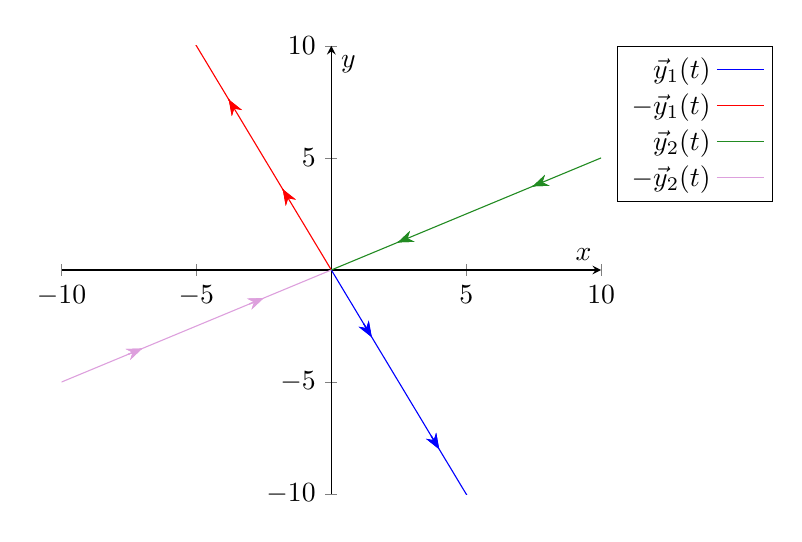
\begin{tikzpicture}[thick,
    curved arrow/.style={arc arrow={to pos #1 with length 2mm and options {}}},
    reversed curved arrow/.style={arc arrow={to pos #1 with length 2mm and options reversed}}]
      \begin{axis}[
        ylabel=$y$,
        xlabel=$x$,
        xmin=-10,xmax=10,
        ymin=-10,ymax=10,
        legend pos=outer north east,
        axis lines=center,
        legend style={legend cell align=right,legend plot pos=right}]

      \addplot[color=blue,domain=0:10,samples=100, curved arrow=0.4,curved arrow=0.15,forget plot] {-2*x};
      \addplot[color=blue,domain=-20:-21,samples=100] {1};
      \addlegendentry{$\vec y_1(t)$}

      \addplot[color=red,domain=-10:0,samples=100,reversed curved arrow=0.85,reversed curved arrow=0.65,forget plot] {-2*x};
      \addplot[color=red,domain=-20:-21,samples=100] {1};
      \addlegendentry{$-\vec y_1(t)$}

      \addplot[color=ForestGreen,domain=0:10,samples=100,reversed curved arrow=0.3,reversed curved arrow=0.8,forget plot] {x/2};
      \addplot[color=ForestGreen,domain=-20:-21,samples=100] {1};
      \addlegendentry{$\vec y_2(t)$}

      \addplot[color=Plum,domain=-10:0,samples=100,curved arrow=0.75,curved arrow=0.3,forget plot] {x/2};
      \addplot[color=Plum,domain=-20:-21,samples=100] {1};
      \addlegendentry{$-\vec y_2(t)$}
      \end{axis}
  \end{tikzpicture}
\end{center}

The system in \textbf{problem 3} has only complex eigenvalues and thus, it has no straight line solutions. Such a system has a spiral equilibrium at the origin. To see the spiral's direction we note that:
\begin{equation*}
  \mathcal R(\lambda)=R(-1\pm i\sqrt{11})=-1<0
\end{equation*}

Meaning the solutions all spiral towards to origin. Next we plug in two test points to help guide our curve. With constants $k_1=k_2=1$ we have at $t=0,\frac{\pi}{2\sqrt{11}}$:
\begin{align*}
  \vec y(0)&=e^0\begin{bmatrix}
    2\cos(0)+\sqrt{11}\sin(0)\\-3\cos(0)
  \end{bmatrix}+e^0\begin{bmatrix}
    -2\sin(0)+\sqrt{11}\cos(0)\\3\sin(0)
  \end{bmatrix}\\
  &=\begin{bmatrix}
    2\\-3
  \end{bmatrix}+\begin{bmatrix}
    \sqrt{11}\\0
  \end{bmatrix}\approx\begin{bmatrix}
    5.317\\-3
  \end{bmatrix}\\
  \vec y\left(\frac{\pi}{2\sqrt{11}}\right)&=e^{\frac{\pi}{2\sqrt{11}}}\begin{bmatrix}
    2\cos\left(\frac{\pi}{2}\right)+\sqrt{11}\sin\left(\frac{\pi}{2}\right)\\-3\cos\left(\frac{\pi}{2}\right)
  \end{bmatrix}+e^{\frac{\pi}{2\sqrt{11}}}\begin{bmatrix}
    -2\sin\left(\frac{\pi}{2}\right)+\sqrt{11}\cos\left(\frac{\pi}{2}\right)\\3\sin\left(\frac{\pi}{2}\right)
  \end{bmatrix}\\
  &=e^{\frac{\pi}{2\sqrt{11}}}\begin{bmatrix}
    \sqrt{11}\\0
  \end{bmatrix}+e^{\frac{\pi}{2\sqrt{11}}}\begin{bmatrix}
    -2\\3
  \end{bmatrix}\approx\begin{bmatrix}
    2.114\\4.817
  \end{bmatrix}
\end{align*}

Now we can graph the phase portrait of the system's spiral sink:
\begin{center}
  \begin{tikzpicture}[thick,
    curved arrow/.style={arc arrow={to pos #1 with length 2mm and options {}}},
    reversed curved arrow/.style={arc arrow={to pos #1 with length 2mm and options reversed}}]
      \begin{axis}[
        ylabel=$y$,
        xlabel=$x$,
        xmin=-10,xmax=10,
        ymin=-10,ymax=10,
        legend pos=outer north east,
        axis lines=center,
        legend style={legend cell align=right,legend plot pos=right}]

        \coordinate[label={270:$(5.317,-3)$},circle,fill,inner sep=1pt] (R) at (axis cs:5.317,-3);
        \coordinate[label={310:$(2.114,4.817)$},circle,fill,inner sep=1pt] (R) at (axis cs:2.114,4.817);
      \end{axis}
  \end{tikzpicture}
\end{center}

For \textbf{problem 4} we have only one straight-line solution: for when $\vec v_0=[1,1]^\top$ (i.e. an eigenvector):
\begin{equation*}
  \vec y_1(t)=e^{-3t}\begin{bmatrix}
    1\\1
  \end{bmatrix},\quad\,\,\,\lambda=-3<0\\
\end{equation*}

Graphing this and and its negative, we see that the origin forms an unstable node equilibrium:
\begin{center}
  \begin{tikzpicture}[thick,
    curved arrow/.style={arc arrow={to pos #1 with length 2mm and options {}}},
    reversed curved arrow/.style={arc arrow={to pos #1 with length 2mm and options reversed}}]
      \begin{axis}[
        ylabel=$y$,
        xlabel=$x$,
        xmin=-10,xmax=10,
        ymin=-10,ymax=10,
        legend pos=outer north east,
        axis lines=center,
        legend style={legend cell align=right,legend plot pos=right}]

      \addplot[color=blue,domain=0:10,samples=100,reversed curved arrow=0.65,reversed curved arrow=0.3,forget plot] {x};
      \addplot[color=blue,domain=-20:-21,samples=100] {1};
      \addlegendentry{$\vec y_1(t)$}

      \addplot[color=red,domain=-10:0,samples=100,curved arrow=0.8,curved arrow=0.4,forget plot] {x};
      \addplot[color=red,domain=-20:-21,samples=100] {1};
      \addlegendentry{$-\vec y_1(t)$}

      \end{axis}
  \end{tikzpicture}
\end{center}

\section*{Problem 6}
\noindent\textbf{Problem:} Let $\vec B$ be a matrix with a repeated zero eigenvalue. Show that $\vec B^2=\vec 0$. Then show that if a matrix $\vec A$ has a repeated eigenvalue $\lambda_0$, then $(\vec A-\lambda_0\vec I)^2=\vec 0$.
\bigskip

\noindent\textbf{Solution:} To prove both statements, we will first prove the Cayley-Hamilton theorem for $2\times2$ matrices. Consider a generic $2\times2$ matrix $\vec M$:
\begin{equation*}
  \vec M=\begin{bmatrix}
    a&b\\c&d
  \end{bmatrix}
\end{equation*}

Now consider its characteristic polynomial $p_{\vec M}(\lambda)$:
\begin{align*}
  p_{\vec M}(\lambda)&=\det(\vec M-\lambda \vec I)\\
  &=\begin{vmatrix} a-\lambda & b \\ c & d-\lambda \end{vmatrix}\\
  &=(a-\lambda)(d-\lambda)-bc\\
  &=\lambda^2-(a+d)\lambda+(ad-bc)
\end{align*}

Now let us adapt this function of a scalar $\lambda$ into a function of a matrix $\vec X$ by multiplying the constants with the identity matrix:

\begin{equation*}
  p_{\vec M}(\vec X)=\vec X^2-(a+d)\vec X+(ad-bc)\vec I
\end{equation*}
\smallskip

The Cayley-Hamilton theorem states that every square matrix satisfies its own characteristic equation. The $2\times2$ case is proven below:
\begin{align*}
  p_{\vec M}(\vec M)&=\vec M^2-(a+d)\vec M+(ad-bc)\vec I\\
  &=\begin{bmatrix}
    a&b\\c&d
  \end{bmatrix}^2-(a+d)\begin{bmatrix}
    a&b\\c&d
  \end{bmatrix}+(ad-bc)\begin{bmatrix}
    1&0\\0&1
  \end{bmatrix}\\
  &=\begin{bmatrix}
    a^2+bc&ab+bd\\ac+cd&bc+d^2
  \end{bmatrix}-\begin{bmatrix}
    a^2+ad&ab+bd\\ac+cd&ad+d^2
  \end{bmatrix}+\begin{bmatrix}
    ad-bc&0\\0&ad-bc
  \end{bmatrix}\\
  &=\begin{bmatrix}
    0&0\\0&0
  \end{bmatrix}=\vec 0
\end{align*}

Armed with this result, we can prove the desired statements. Consider a $2\times2$ matrix $\vec B$ with a single repeated eigenvalue of $\lambda_0=0$. The characteristic polynomial of this matrix is given by:

\begin{equation*}
  p_{\vec B}(\vec X)=(\vec X-\lambda_0\vec I)(\vec X-\lambda_0\vec I)=\vec X^2
\end{equation*}
\smallskip

Plugging our matrix $\vec B$ into the polynomial, the Cayley-Hamilton theorem tells us:

\begin{equation*}
  p_{\vec B}(\vec B)=\tcbhighmath[boxrule=0.4pt,colframe=blue,colback=blue!10!white]{\vec B^2=\vec 0}
\end{equation*}
\smallskip

Now consider a $2\times2$ matrix $\vec A$ with a repeated eigenvalue $\lambda_0$. Its characteristic polynomial is given by:

\begin{equation*}
  p_{\vec A}(\vec X)=(\vec X-\lambda_0\vec I)(\vec X-\lambda_0\vec I)=(\vec X-\lambda_0\vec I)^2
\end{equation*}
\smallskip

And once again, plugging our matrix $\vec A$ into the polynomial, the Cayley-Hamilton theorem tells us:

\begin{equation*}
  p_{\vec A}(\vec A)=\tcbhighmath[boxrule=0.4pt,colframe=blue,colback=blue!10!white]{(\vec A-\lambda_0\vec I)^2=\vec 0}
\end{equation*}

\section*{Problem 7}
\noindent\textbf{Problem:} Given the following family of systems with parameter $a$:

\begin{equation*}
  \der[\vec y]=\underbrace{\begin{bmatrix}
    a&a^2+a\\1&a
  \end{bmatrix}}_{\vec X}\vec y
\end{equation*}

sketch the corresponding curve in the trace-determinant plane. Identify the values of $a$ where the type of the system changes, i.e. the bifurcation values of the family.
\bigskip

\noindent\textbf{Solution:} First we compute the trace and determinant of the given matrix:
\begin{align*}
  \tr{\vec X_a}&=2a\\
  \det(\vec X_a)&=a^2-a^2-a=-a
\end{align*}

% And so the solution curve is given by the following set of vectors:
% \begin{align*}
%   (\det{\vec X},\tr{\vec X})&=(2a,-a)\\
%     &=a(2,-1)\\
%     &=\text{Span}\left\{\begin{bmatrix}
%     2\\-1
%   \end{bmatrix}\right\}
% \end{align*}

Now we can graph this and the repeated root parabola on the trace-determinant plane:

\begin{center}
  \begin{tikzpicture}
      \begin{axis}[
        ylabel=$\det{}$,
        xlabel=$\text{tr}$,
        xmin=-3,xmax=3,
        ymin=-3,ymax=3,
        legend pos=outer north east,
        axis lines=center,
        legend style={legend cell align=right,legend plot pos=right}]

      \addplot[color=blue,domain=-3:3,samples=100] {x^2/4};
      \addlegendentry{$\det{}=\frac{\text{tr}^2}{4}$}

      \addplot[color=red,domain=-3:3,samples=100] {-x/2};
      \addlegendentry{$\forall a\,\,(2a,-a)$}
      \coordinate[label={60:$(2,-1)$},circle,fill,inner sep=1pt] (R) at (axis cs:-2,1);
      \coordinate[label={70:$(0,0)$},circle,fill,inner sep=1pt] (R) at (axis cs:0,0);
      \end{axis}
  \end{tikzpicture}
  \end{center}

  A bifurcation occurs when the solution curve intersects the parabola or either of the axes. The two points this happens at translate to the following bifurcation values:
  \begin{align*}
    (0,0)&=a_0(2,-1)\rightarrow a_0=0\\
    (-2,1)&=a_1(2,-1)\rightarrow a_1=-1
  \end{align*}

  \tcbox[boxrule=0.4pt,colframe=blue,colback=blue!10!white]{And so the bifurcation values of the system are $a_0=0$ and $a_1=-1$.}

\end{document}